\documentclass[a4paper, 14pt]{extarticle}

% Поля
%--------------------------------------
\usepackage{geometry}
\geometry{a4paper,tmargin=2cm,bmargin=2cm,lmargin=3cm,rmargin=1cm}
%--------------------------------------


%Russian-specific packages
%--------------------------------------
\usepackage[T2A]{fontenc}
\usepackage[utf8]{inputenc} 
\usepackage[english, main=russian]{babel}
%--------------------------------------

\usepackage{textcomp}

% Красная строка
%--------------------------------------
\usepackage{indentfirst}               
%--------------------------------------             


%Graphics
%--------------------------------------
\usepackage{graphicx}
\graphicspath{ {./images/} }
\usepackage{wrapfig}
%--------------------------------------

% Полуторный интервал
%--------------------------------------
\linespread{1.3}                    
%--------------------------------------

%Выравнивание и переносы
%--------------------------------------
% Избавляемся от переполнений
\sloppy
% Запрещаем разрыв страницы после первой строки абзаца
\clubpenalty=10000
% Запрещаем разрыв страницы после последней строки абзаца
\widowpenalty=10000
%--------------------------------------

%Списки
\usepackage{enumitem}

%Подписи
\usepackage{caption} 

%Гиперссылки
\usepackage{hyperref}

\hypersetup {
	unicode=true
}

%Рисунки
%--------------------------------------
\DeclareCaptionLabelSeparator*{emdash}{~--- }
\captionsetup[figure]{labelsep=emdash,font=onehalfspacing,position=bottom}
%--------------------------------------

\usepackage{tempora}
\usepackage{amsmath}
\usepackage{color}
\usepackage{listings}
\lstset{
  belowcaptionskip=1\baselineskip,
  breaklines=true,
  frame=L,
  xleftmargin=\parindent,
  language=Python,
  showstringspaces=false,
  basicstyle=\footnotesize\ttfamily,
  keywordstyle=\bfseries\color{blue},
  commentstyle=\itshape\color{purple},
  identifierstyle=\color{black},
  stringstyle=\color{red},
}

%--------------------------------------
%			НАЧАЛО ДОКУМЕНТА
%--------------------------------------

\begin{document}

%--------------------------------------
%			ТИТУЛЬНЫЙ ЛИСТ
%--------------------------------------
\begin{titlepage}
\thispagestyle{empty}
\newpage


%Шапка титульного листа
%--------------------------------------
\vspace*{-60pt}
\hspace{-65pt}
\begin{minipage}{0.3\textwidth}
\hspace*{-20pt}\centering

\includegraphics[width=\textwidth]{emblem}
\end{minipage}
\begin{minipage}{0.67\textwidth}\small \textbf{
\vspace*{-0.7ex}
\hspace*{-6pt}\centerline{Министерство науки и высшего образования Российской Федерации}
\vspace*{-0.7ex}
\centerline{Федеральное государственное бюджетное образовательное учреждение }
\vspace*{-0.7ex}
\centerline{высшего образования}
\vspace*{-0.7ex}
\centerline{<<Московский государственный технический университет}
\vspace*{-0.7ex}
\centerline{имени Н.Э. Баумана}
\vspace*{-0.7ex}
\centerline{(национальный исследовательский университет)>>}
\vspace*{-0.7ex}
\centerline{(МГТУ им. Н.Э. Баумана)}}
\end{minipage}
%--------------------------------------

%Полосы
%--------------------------------------
\vspace{-25pt}
\hspace{-35pt}\rule{\textwidth}{2.3pt}

\vspace*{-20.3pt}
\hspace{-35pt}\rule{\textwidth}{0.4pt}
%--------------------------------------

\vspace{1.5ex}
\hspace{-35pt} \noindent \small ФАКУЛЬТЕТ\hspace{80pt} <<Информатика и системы управления>>

\vspace*{-16pt}
\hspace{47pt}\rule{0.83\textwidth}{0.4pt}

\vspace{0.5ex}
\hspace{-35pt} \noindent \small КАФЕДРА\hspace{50pt} <<Теоретическая информатика и компьютерные технологии>>

\vspace*{-16pt}
\hspace{30pt}\rule{0.866\textwidth}{0.4pt}
  
\vspace{11em}

\begin{center}
\Large {\bf Лабораторная работа № 4} \\ 
\large {\bf по курсу <<Языки и методы программирования>>} \\ 
\large <<Реализация итераторов в языке Java>>
\end{center}\normalsize

\vspace{8em}


\begin{flushright}
  {Студент группы ИУ9-21Б Хромов М.А.\hspace*{15pt} \\
  \vspace{2ex}
  Преподаватель Посевин Д. П.\hspace*{15pt}}
\end{flushright}

\bigskip

\vfill
 

\begin{center}
\textsl{Москва 2025}
\end{center}
\end{titlepage}
%--------------------------------------
%		КОНЕЦ ТИТУЛЬНОГО ЛИСТА
%--------------------------------------

\renewcommand{\ttdefault}{pcr}

\setlength{\tabcolsep}{3pt}
\newpage
\section{Цель}\label{Sect::task}
\par
Целью данной работы является изучение обобщённых итераторов и экземплярных вложенных классов языка Java.


\section{Задание}\label{Sect::task}
\par
Во время выполнения лабораторной работы требуется разработать на языке Java один из классов, перечисленных в таблицах 1 – 7. Класс должен реализовывать интерфейс Iterable. 
\par
Объект разрабатывемого класса должен быть изменяемым, то есть в нём надо так или иначе предусмотреть возможность изменения внутреннего состояния. 
\par
В методе main вспомогательного класса Test нужно продемонстрировать работоспособность разработанного класса. 
\par
Во время выполнения лабораторной работы требуется разработать на языке Java один из классов, перечисленных в таблицах 1 – 7. Класс должен реализовывать интерфейс Iterable. 
\par
Объект разрабатывемого класса должен быть изменяемым, то есть в нём надо так или иначе предусмотреть возможность изменения внутреннего состояния. 
\par
В методе main вспомогательного класса Test нужно продемонстрировать работоспособность разработанного класса. 

\section{Индивидуальный вариант}
\par
Вариант 2 + Вариант 6
\par 
Параметризованная типовым параметром T последовательность контейнеров, классы которых реализуют интерфейс Iterable (итератор – «конкатенация» итераторов контейнеров). 
\par
Класс, представляющий множество арифметических прогрессий, с итераторам по числам, принадлежащим этим арифметическим прогрессиям. Итератор должен выдавать числа в порядке возрастания. 

\section {Практическая реализация}
Исходный код программы представлен в листингах~\ref{lst:code1}--~\ref{lst:code4}.
\begin{figure}[!htb]
\begin{lstlisting}[language={},caption={Основной класс для варинта 2 (IntSet)},label={lst:code1}]
import java.util.Iterator;
import java.util.List;
import java.util.NoSuchElementException;

public class JoinedIterable<T> implements Iterable<T> {
    private final List<Iterable<T>> iterables;

    public JoinedIterable(List<Iterable<T>> iterables) {
        this.iterables = iterables;
    }

    public Iterator<T> iterator() {
        return new JoinedIterator();
    }

    private class JoinedIterator implements Iterator<T> {
        private int currentIterableIndex = 0;
        private Iterator<T> currentIterator;

        public JoinedIterator() {
            if (!iterables.isEmpty()) {
                currentIterator = iterables.get(0).iterator();
            }
        }
        public boolean hasNext() {
            while (currentIterableIndex < iterables.size()) {
                if (currentIterator.hasNext()) {
                    return true;
                } else {
                    currentIterableIndex++;
                    if (currentIterableIndex < iterables.size()) {
                        currentIterator = iterables.get(currentIterableIndex).iterator();
                    }
                }
            }
            return false;
        }
        public T next() {
            if (!hasNext()) {
                throw new NoSuchElementException();
            }
            return currentIterator.next();
        }
    }
}


\end{lstlisting}
\end{figure}
\newpage
\begin{figure}[!htb]
\begin{lstlisting}[language={},caption={Основной класс для варианта 6 (SymmetricMatrix)},label={lst:code2}]
import java.util.Iterator;
import java.util.List;
import java.util.NoSuchElementException;

public class JoinedIterable<T> implements Iterable<T> {
    private final List<Iterable<T>> iterables;

    public JoinedIterable(List<Iterable<T>> iterables) {
        this.iterables = iterables;
    }

    public Iterator<T> iterator() {
        return new JoinedIterator();
    }

    private class JoinedIterator implements Iterator<T> {
        private int currentIterableIndex = 0;
        private Iterator<T> currentIterator;

        public JoinedIterator() {
            if (!iterables.isEmpty()) {
                currentIterator = iterables.get(0).iterator();
            }
        }
        public boolean hasNext() {
            while (currentIterableIndex < iterables.size()) {
                if (currentIterator.hasNext()) {
                    return true;
                } else {
                    currentIterableIndex++;
                    if (currentIterableIndex < iterables.size()) {
                        currentIterator = iterables.get(currentIterableIndex).iterator();
                    }
                }
            }
            return false;
        }
        public T next() {
            if (!hasNext()) {
                throw new NoSuchElementException();
            }
            return currentIterator.next();
        }
    }
}


\end{lstlisting}
\end{figure}
\newpage
\begin{figure}[!htb]
\begin{lstlisting}[language={},caption={Тестовый класс для варинта 2 },label={lst:code3}]
import java.util.ArrayList;
import java.util.Arrays;
import java.util.List;

public class Test {
    public static void main(String[] args) {
        List<Integer> list1 = Arrays.asList(1, 2, 3);
        List<Integer> list2 = Arrays.asList(4, 5);
        List<Integer> list3 = Arrays.asList(6, 7, 8, 9);

        List<Iterable<Integer>> iterables = new ArrayList<>();
        iterables.add(list1);
        iterables.add(list2);
        iterables.add(list3);

        JoinedIterable<Integer> joined = new JoinedIterable<>(iterables);

        System.out.println("Элементы после конкатенации:");
        for (int x : joined) {
            System.out.print(x + " ");
        }
        System.out.println();
    }
}


\end{lstlisting}
\end{figure}
\newpage
\begin{figure}[!htb]
\begin{lstlisting}[language={},caption={Тестовый класс для варинта 6},label={lst:code4}]
public class Test {
    public static void main(String[] args) {
        ArithmeticProgressions ap = new ArithmeticProgressions();

        ap.addProgression(1, 3);
        ap.addProgression(2, 2);
        ap.addProgression(5, 5);

        System.out.println("Числа из прогрессий в порядке возрастания:");
        for (int num : ap) {
            if (num > 20) break;
            System.out.print(num + " ");
        }
    }
}


\end{lstlisting}
\end{figure}
\clearpage
\newpage

\section{}
\begin{center}
    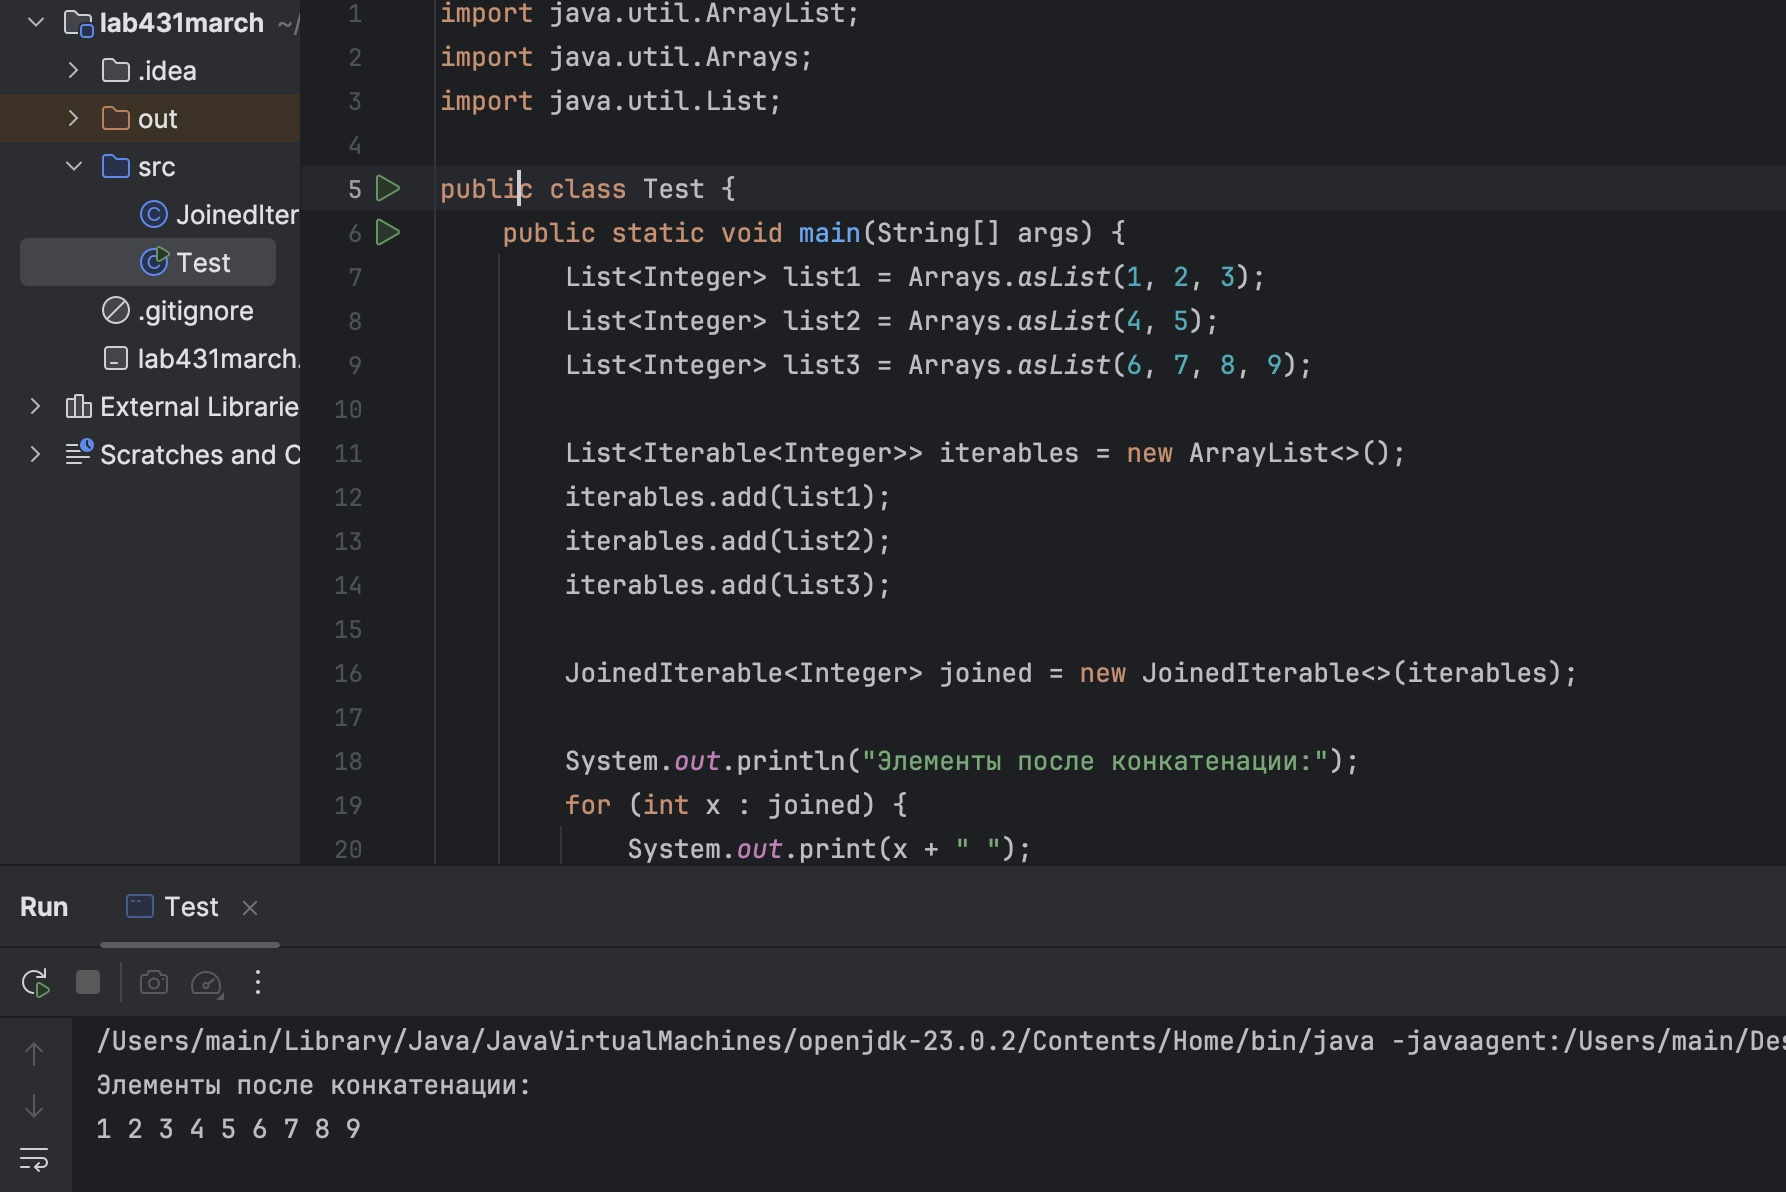
\includegraphics[width=0.8\textwidth]{фото6.jpeg}
    \captionof{figure}{Запуск программы1}
\end{center}
\newpage


\section{}
\begin{center}
    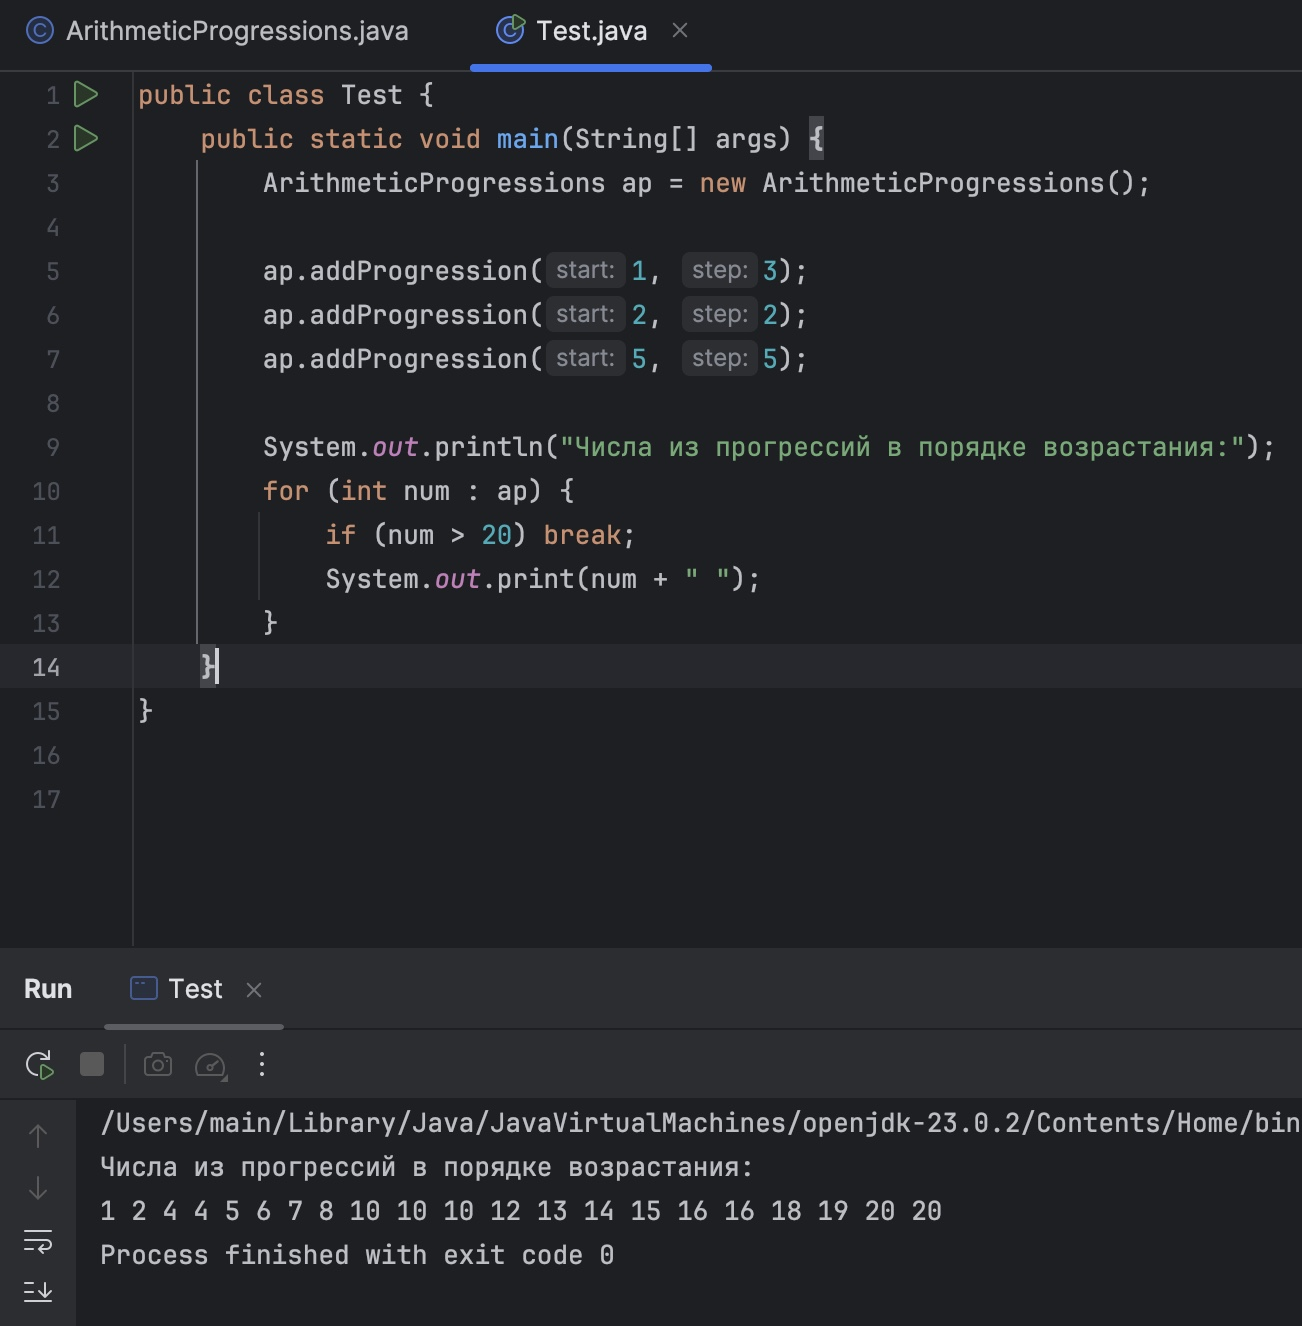
\includegraphics[width=0.8\textwidth]{фото7.jpeg}
    \captionof{figure}{Запуск программы2}
\end{center}
\newpage
\section{Вывод}
В ходе выполнения лабораторной работы были разработаны два класса на языке Java, реализующие интерфейс Iterable:

JoinedIterable<T> — для конкатенации итераторов из коллекции контейнеров (вариант 2).

ArithmeticProgressions — для работы с множеством арифметических прогрессий и итерации по их элементам в порядке возрастания (вариант 6).

Для каждого класса были созданы тестовые сценарии, подтверждающие корректность работы:

Для JoinedIterable продемонстрирована последовательная итерация по элементам нескольких списков.

Для ArithmeticProgressions показана генерация чисел из прогрессий с выводом в отсортированном порядке.

Результаты выполнения программы соответствуют ожиданиям: итераторы корректно обрабатывают данные, а изменяемость внутреннего состояния объектов обеспечивается методами добавления новых контейнеров (JoinedIterable) и прогрессий (ArithmeticProgressions). Работа с обобщенными типами и вложенными классами освоена на практике.

\end{document}